% Contributions are much appreciated, in order to contribute to this project, head over to this repository:
% https://github.com/bshramin/uofa-eng-assignment

\documentclass[11pt,letterpaper]{article}
\textwidth 6.5in
\textheight 9.in
\oddsidemargin 0in
\headheight 0in
\usepackage{graphicx}
\usepackage{fancybox}
\usepackage[utf8]{inputenc}
\usepackage{epsfig,graphicx}
\usepackage{multicol,pst-plot}
\usepackage{pstricks}
\usepackage{amsmath}
\usepackage{amsfonts}
\usepackage{amssymb}
\usepackage{eucal}
\usepackage[left=2cm,right=2cm,top=2cm,bottom=2cm]{geometry}
\usepackage{esvect}
\pagestyle{empty}
\DeclareMathOperator{\tr}{Tr}
\newcommand*{\op}[1]{\check{\mathbf#1}}
\newcommand{\bra}[1]{\langle #1 |}
\newcommand{\ket}[1]{| #1 \rangle}
\newcommand{\braket}[2]{\langle #1 | #2 \rangle}
\newcommand{\mean}[1]{\langle #1 \rangle}
\newcommand{\opvec}[1]{\check{\vec #1}}
\renewcommand{\sp}[1]{$${\begin{split}#1\end{split}}$$}

\usepackage{lipsum}

\usepackage{listings}
\usepackage{color}
\usepackage{wrapfig}
\usepackage[shortlabels]{enumitem}

\definecolor{codegreen}{rgb}{0,0.6,0}
\definecolor{codegray}{rgb}{0.5,0.5,0.5}
\definecolor{codepurple}{rgb}{0.58,0,0.82}
\definecolor{backcolour}{rgb}{0.95,0.95,0.92}

\lstdefinestyle{mystyle}{
	backgroundcolor=\color{backcolour},   
	commentstyle=\color{codegreen},
	keywordstyle=\color{magenta},
	numberstyle=\tiny\color{codegray},
	stringstyle=\color{codepurple},
	basicstyle=\footnotesize,
	breakatwhitespace=false,         
	breaklines=true,                 
	captionpos=b,                    
	keepspaces=true,                 
	numbers=left,                    
	numbersep=5pt,                  
	showspaces=false,                
	showstringspaces=false,
	showtabs=false,                  
	tabsize=2
}

\lstset{style=mystyle}

\begin{document}
\pagestyle{plain}

\begin{flushleft}
Estudiante: Fabio Quimbay\\
Email: fabio.quimbay883@comunidadunir.net\\
Profesor: Miguel Ángel Cabeza\\
Fecha: Noviembre 11 de 2022\\
\end{flushleft}

\begin{flushright}\vspace{-20mm}

\includegraphics[height=2cm]{logo.png}
\end{flushright}
 
\begin{center}\vspace{0cm}
\textbf{\large PER5786 2022-2023  Física 1 (GFI) - PER5786 2022-2023}\\
 Tema 3 - Movimientos elementales
\end{center}

 
\rule{\linewidth}{0.1mm}
%%%%%%%%%%%%%%%%%%%%%%%%%%%%%%%%%%%%%%%%%%%%%%%%%%%%%%%%%%%%%%%%%%%%%%%%

\bigskip
\bigskip

%%%%%%%%%%%%%%%%%%%%
\textbf{Problema propuesto 4}\\

\begin{wrapfigure}{r}{0.25\textwidth}
\begin{center}
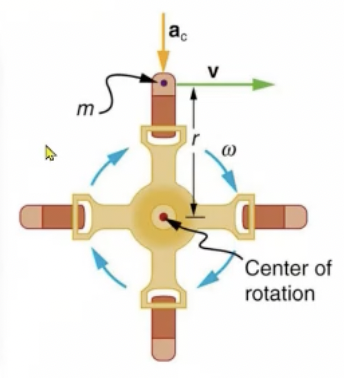
\includegraphics[width=0.25\textwidth]{problema_4.png}
\end{center}
\end{wrapfigure}

Las centrifugadoras industriales son empleadas, p.ej., en el proceso de purificación de vacunas. Calcula el radio de giro del rotor de una “ultracentrifugadora” cuyo fabricante indica que es capaz de alcanzar 150,000 rpm (revoluciones por minuto) y 1,048,000 veces la aceleración de la gravedad ($9,8 m/s^2$).\\

\textbf{Formulas base:}\\

Se tomarán las siguientes formulas base del MCUA:

\begin{align}
\boxed{ \vec{a_{c}} = \frac{v^2}{r} = \frac{(w \cdot r)^2}{r} = w^2 \cdot r}
\end{align}

\textbf{Solución:}\\

Se requiere poder expresar las unidades dadas en rpm en su equivalente en radianes, como sigue:

\begin{align}
\omega &= \frac{150,000\,vueltas}{1\,min} = \frac{2 \cdot \pi \cdot 150,000}{60\,s} = 500 \cdot \pi\,rad/s \approx 15,708\,rad/s
\end{align}

Y ahora, al despejar $r$ de la formula base, obtenemos:

\begin{align}
r = \frac{a_{c}}{w^2} = \frac{9.8 \times 1,048,000}{15,708^2} = 0.041624 \approx 4.1624 \times 10^{-2}\,m.
\end{align}

Por lo que, el radio de giro ($r$) corresponde a $4.1624 \times 10^{-2}\,m.$

%%%%%%%%%%%%%%%%%%%%

\end{document}

